\documentclass[14pt]{extarticle}

\usepackage[utf8]{inputenc}
\usepackage[T2A,T1]{fontenc}
\usepackage[russian]{babel}
\usepackage[a4paper,lmargin=3cm,rmargin=2cm,tmargin=2cm,bmargin=2cm]{geometry}
\usepackage[ddmmyyyy]{datetime}
\usepackage{indentfirst}
\usepackage{hyperref}
\usepackage{graphicx}
\graphicspath{{./images/}}

\usepackage{minted}

\usepackage{titlesec}
\titleformat{\section}{\normalfont\bfseries\centering}{\thesection}{1em}{}
\titleformat{\subsection}{\normalfont\bfseries}{\thesubsection}{1em}{}
\usepackage{setspace}
\singlespacing
%\onehalfspacing
%\doublespacing
\setlength{\parindent}{1.25cm}
\let\oldsection\section
\renewcommand\section{\clearpage\oldsection}

\usepackage[backend=biber]{biblatex}
\addbibresource{~/texdoc/bibl.bib}
\input{~/texdoc/unibind.tex}

\usepackage{pgf}
\usepackage{tikz}
\usetikzlibrary{arrows,automata}
\usetikzlibrary{positioning}

\tikzset{
	state/.style={
		rectangle,
		draw=black, very thick,
		anchor=west, align=left,
		text width=6cm,
	},
}
\usepackage{csquotes}

\usepackage{multirow} %\multirow{NUMBER_OF_ROWS}{WIDTH}{CONTENT}
% \multicolumn{NUMBER_OF_COLUMNS}{ALIGNMENT}{CONTENT}

\begin{document}
\unititle
{\klgtu}
{\fapu}
{\suvt}
{Лабораторная Работа}
{По дисциплине: «Сетевые информационные технологии и программирование» \par Работа 5}
{Доцент}
{Ломакина Г.В.}
{ст. гр. 18-ВТ}
{Поляков Л.Д.}

\tableofcontents


\section{Ход Разработки}

\begin{figure}[h]
    \centering
	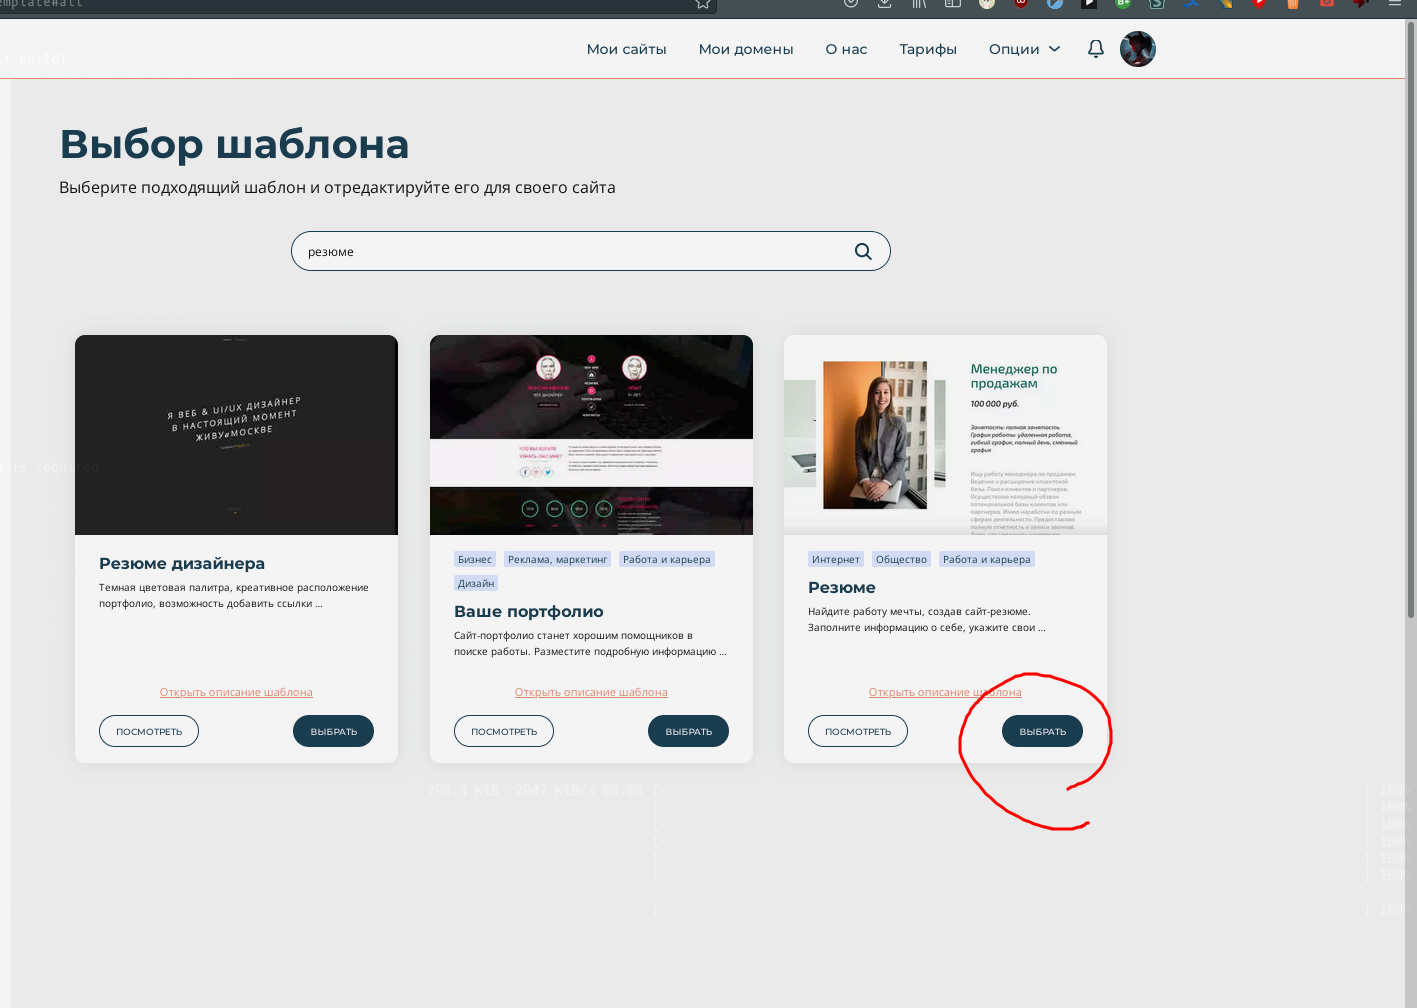
\includegraphics[width=0.9\textwidth, angle=0]{2021-12-12_18-00}
    \caption{Разработка WEB\-страницы \#1}
    \label{fig:html1}
\end{figure}

\begin{figure}[h]
    \centering
	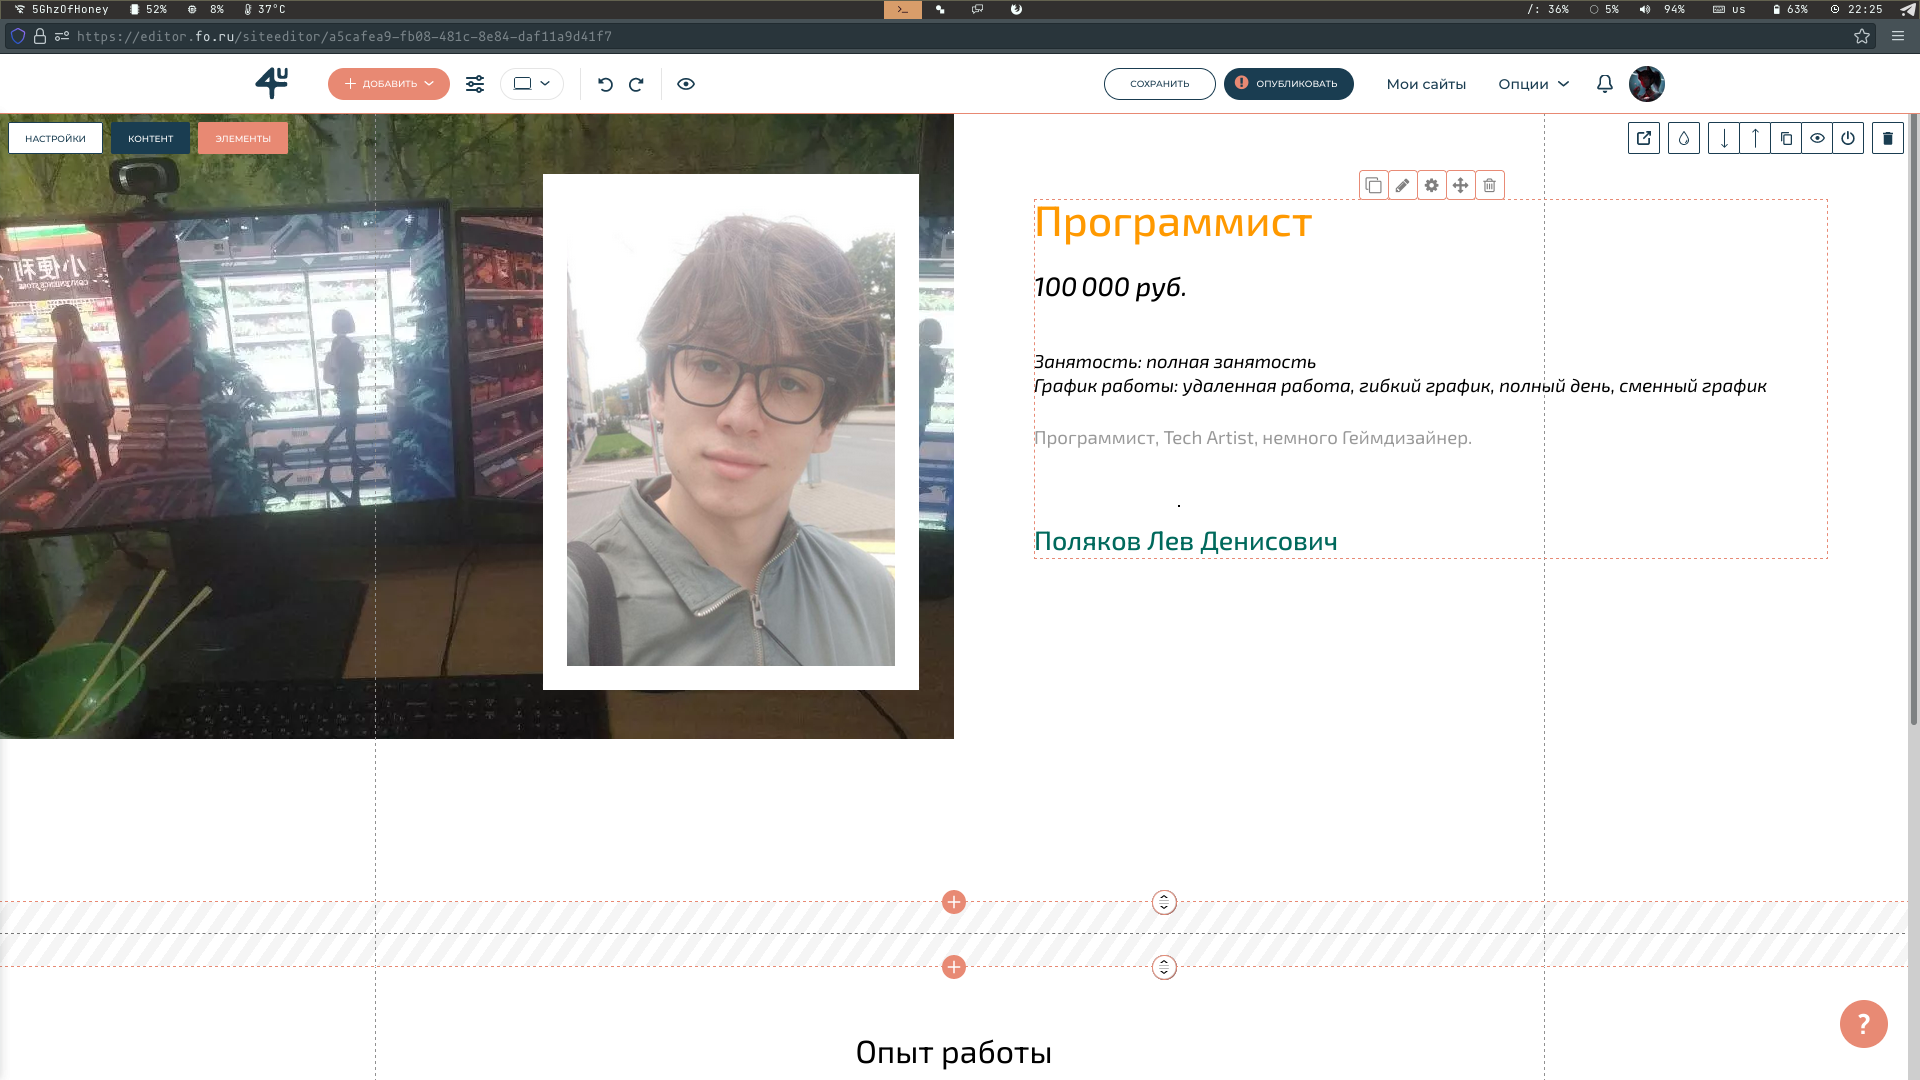
\includegraphics[width=0.9\textwidth, angle=0]{2021-10-19-22-25-30}
    \caption{Разработка WEB\-страницы \#2}
    \label{fig:html2}
\end{figure}

\begin{figure}[h]
    \centering
	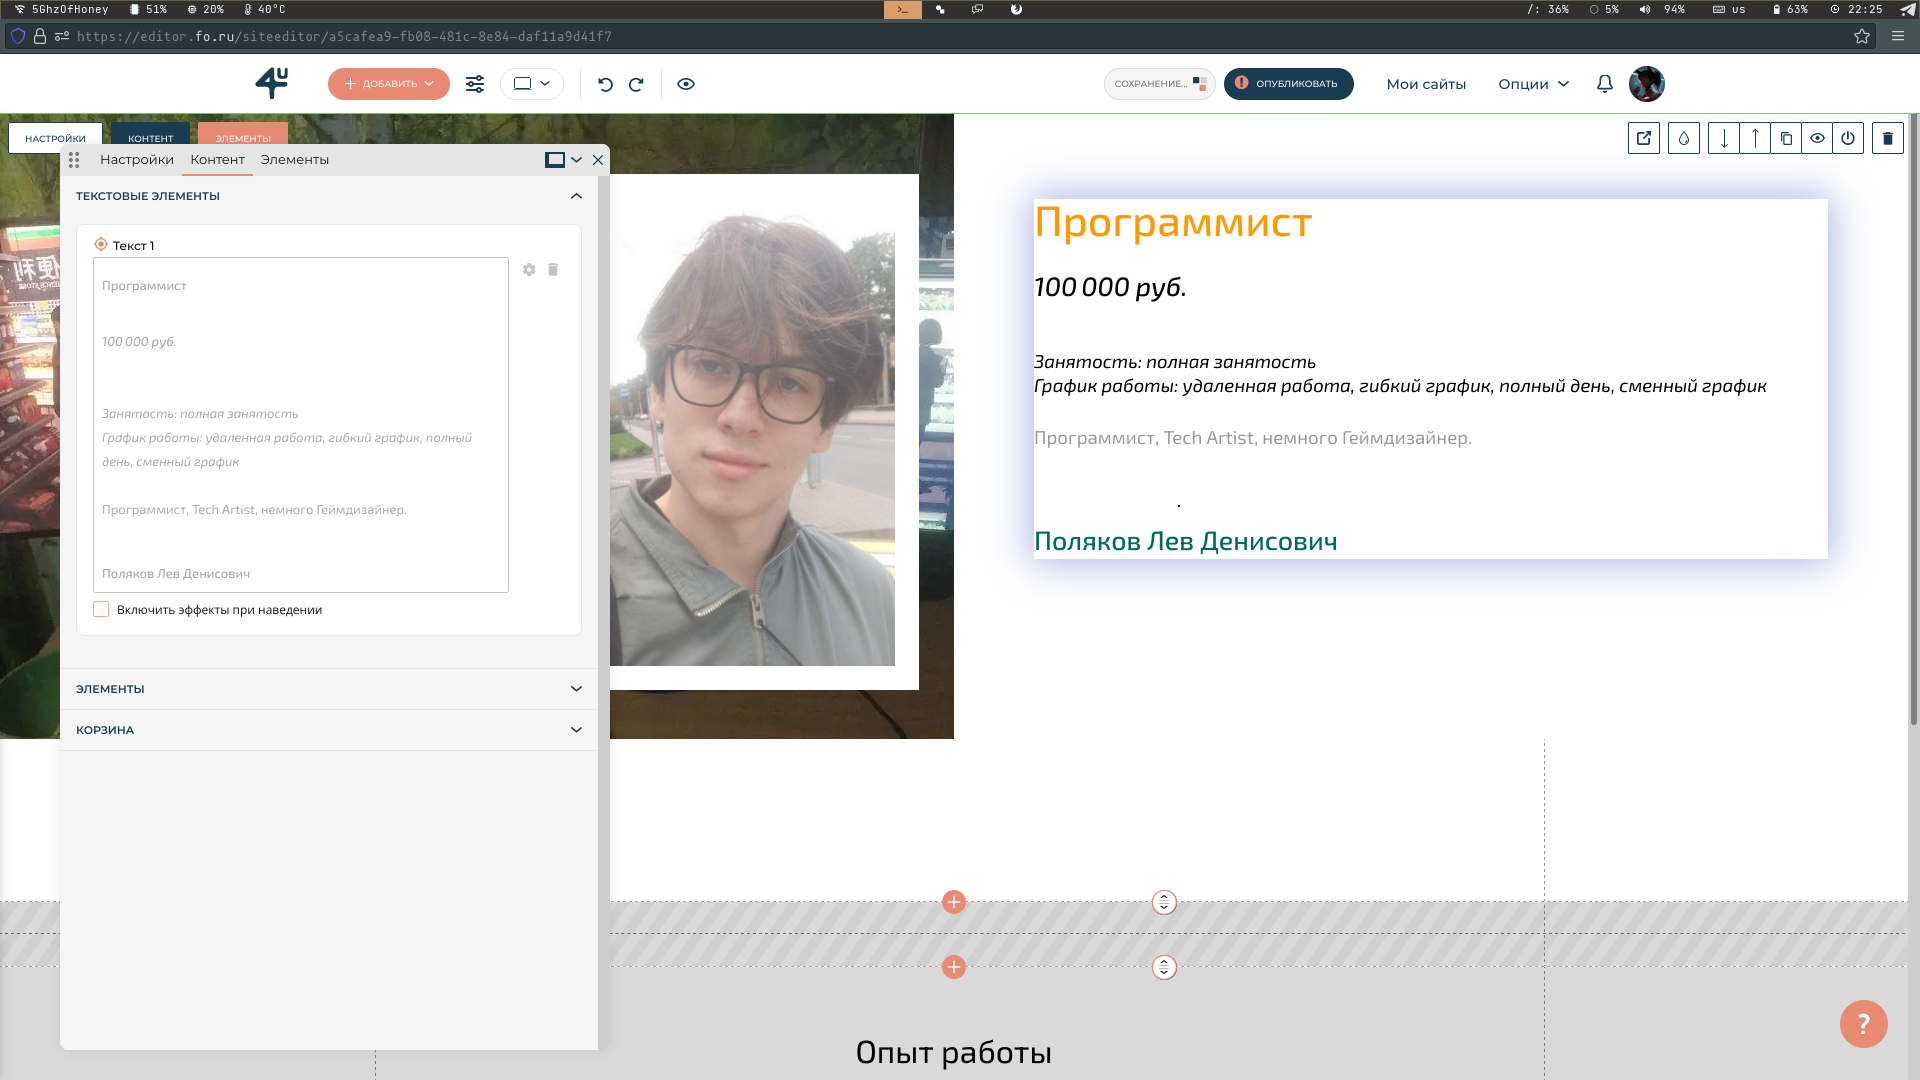
\includegraphics[width=0.9\textwidth, angle=0]{2021-10-19-22-25-47}
    \caption{Разработка WEB\-страницы \#3}
    \label{fig:html3}
\end{figure}

\begin{figure}[h]
    \centering
	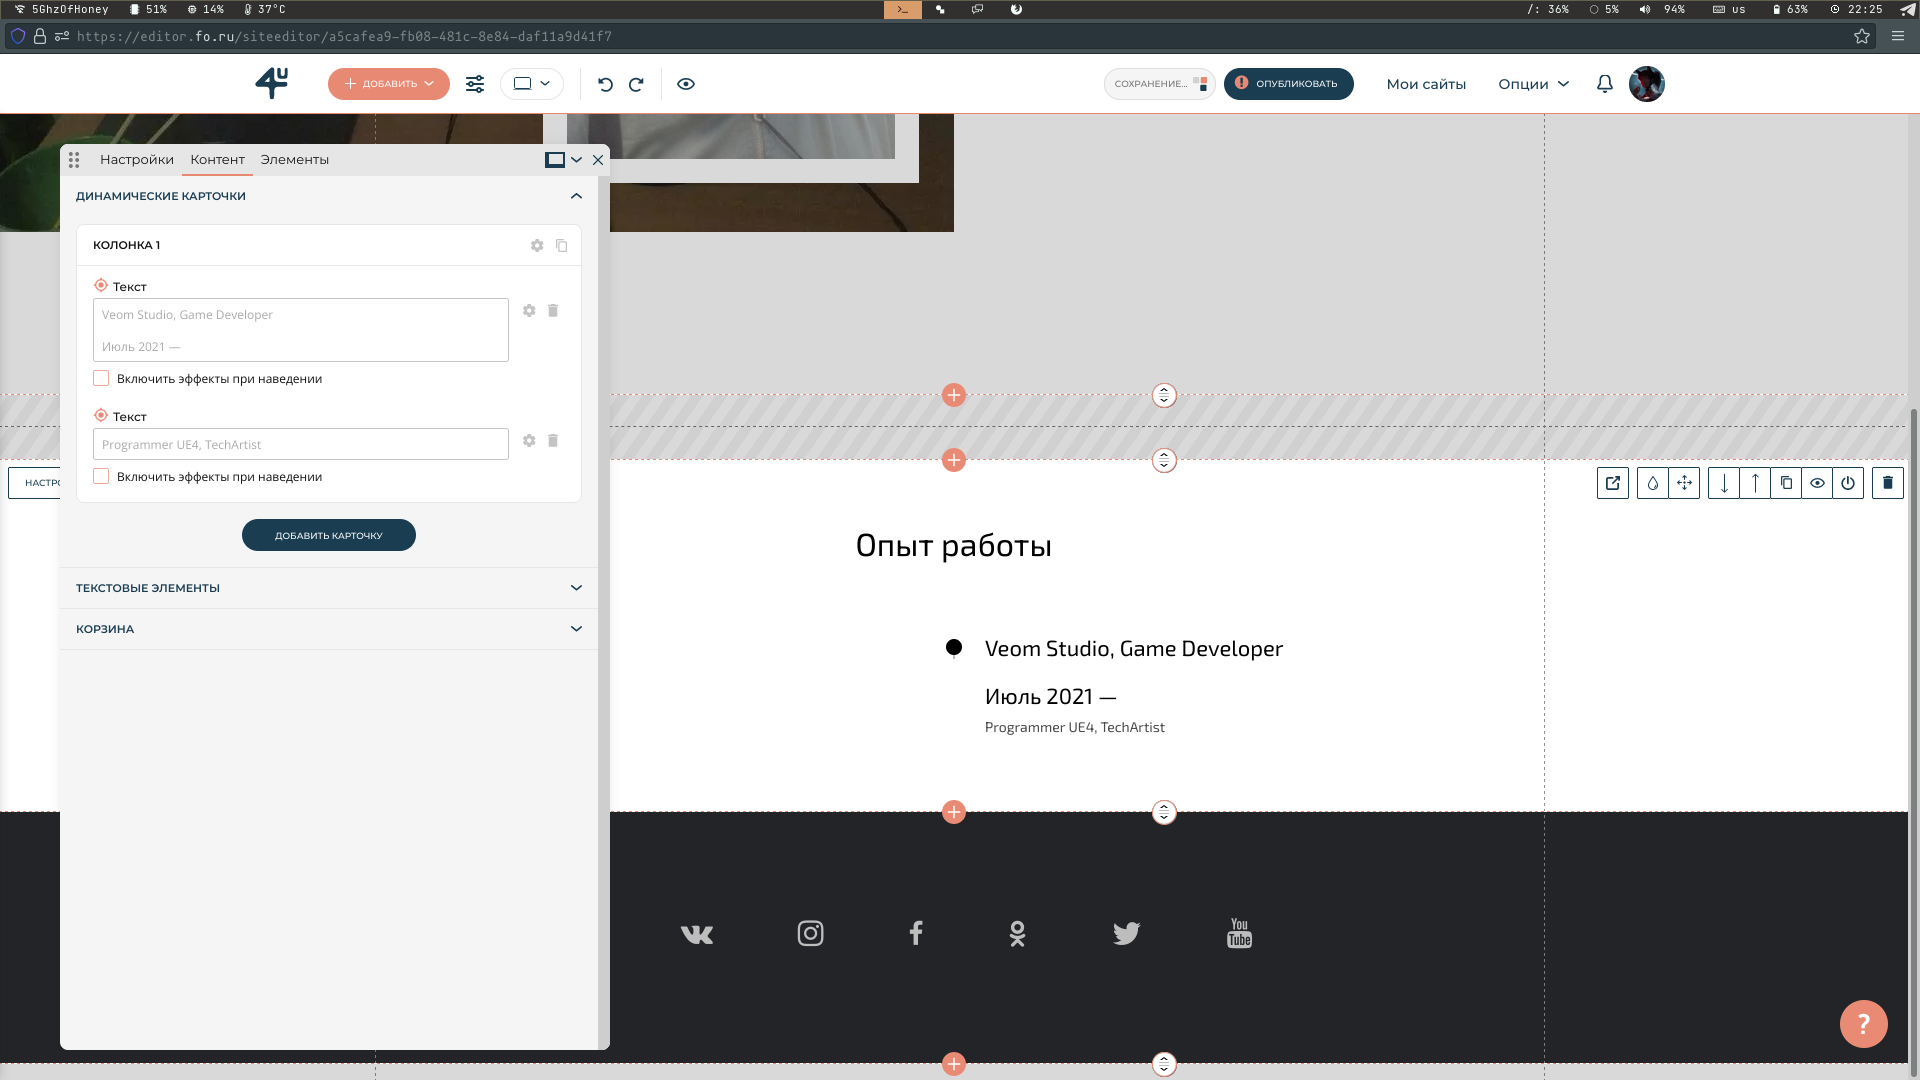
\includegraphics[width=0.9\textwidth, angle=0]{2021-10-19-22-25-56}
    \caption{Разработка WEB\-страницы \#4}
    \label{fig:html4}
\end{figure}

\begin{figure}[h]
    \centering
	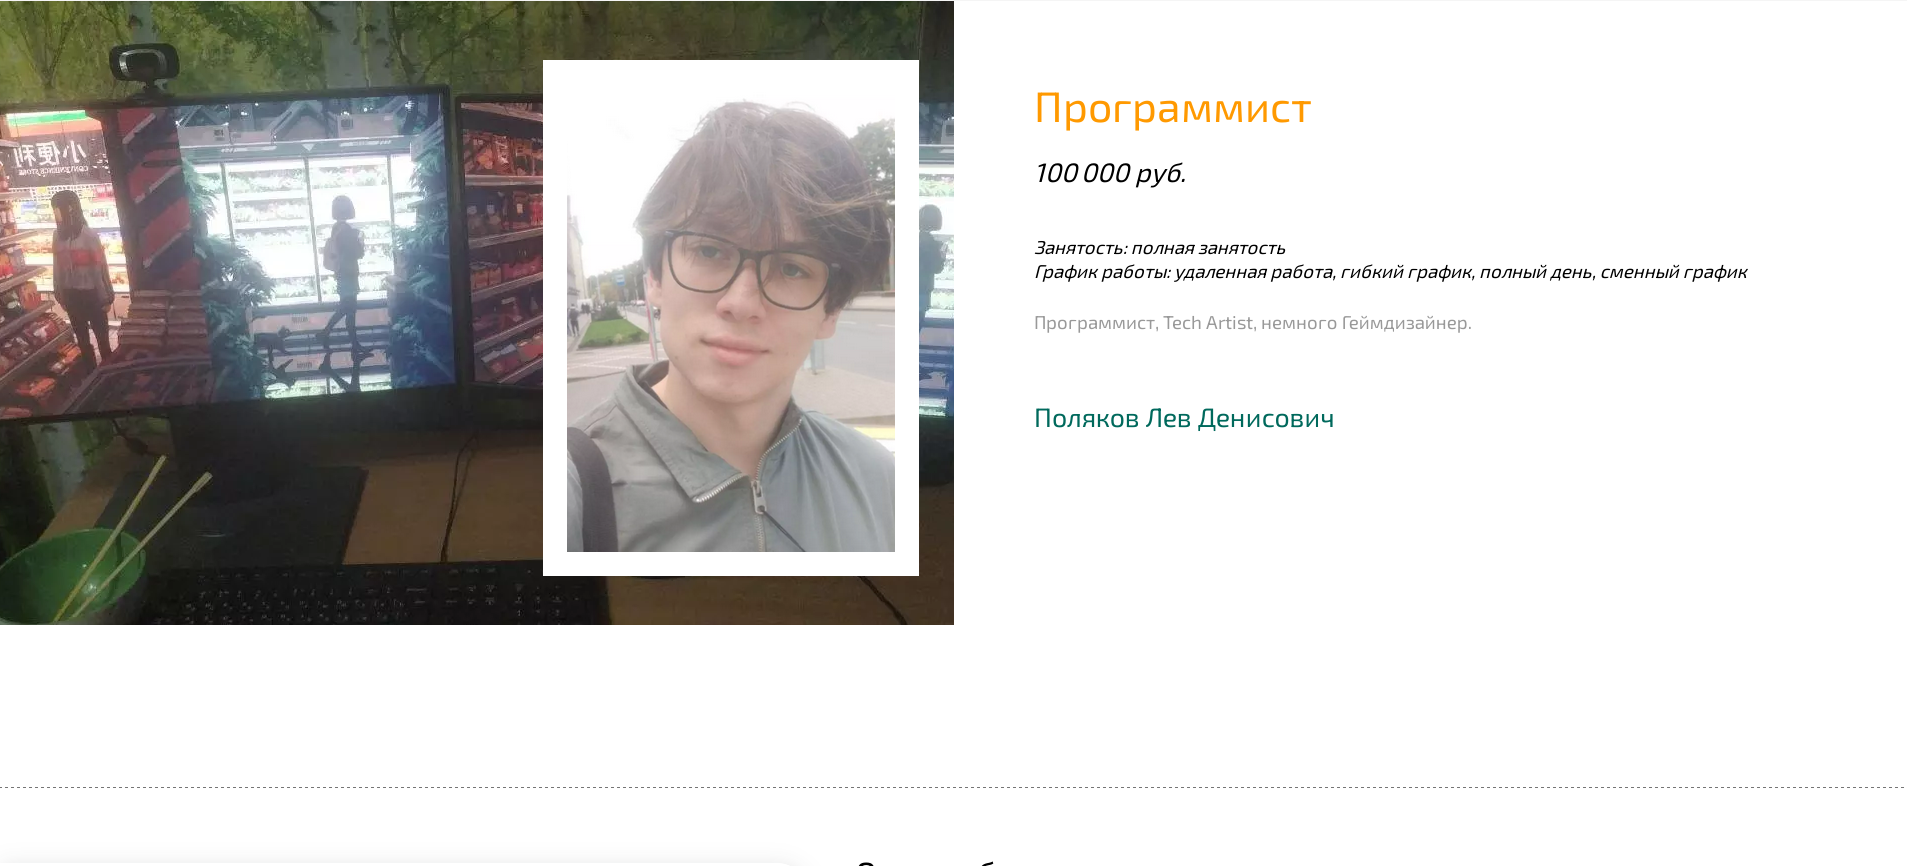
\includegraphics[width=0.9\textwidth, angle=0]{2021-12-12_18-29}
    \caption{Итоговая WEB\-страница}
    \label{fig:html4}
\end{figure}

\end{document}
